\def\uds#1{#1}
\def\perm#1{\pi_k(#1)}

\section{Optimization}
\label{sec:optimization}

We now describe in detail the optimization algorithm for the additive
convex regression stage.  The second decoupled concave regression stage
follows a very similar procedure.

Let $\bds{x}_{i}\in\mathbb{R}^{p}$ be the covariate, let $y_{i}$ be
the response and let $\epsilon_{i}$ be the mean zero noise. The
regression function $f(\cdot)$ we estimate is the sum of
univariate functions $f_{k}(\cdot)$ in each variable dimension and a scalar
offset $\mu$.  We impose additional constraints that each
function $f_{k}(\cdot)$ is convex, which can be
represented by its supporting hyperplanes, i.e.,
\begin{equation}\label{hyper}
      f_{i'k} \geq f_{ik} + \beta_{ik}(x_{i'k}-x_{ik}) \quad
      \textrm{for all $i,i' = 1,\ldots, n$,}
\end{equation}
where $f_{ik}\coloneqq f_{k}(x_{ik})$ is the function value and $\beta_{ik}$ is a
subgradient at point $x_{ik}$. This ostensibly requires $O(n^2 p)$ constraints to
impose the supporting hyperplane constraints.
In fact, only $O(np)$
constraints suffice, since univariate convex functions are
characterized by the condition that the subgradient, which is a scalar, must
increase monotonically. This observation leads to the  optimization
\begin{equation}
\begin{split}
       \min_{f,\beta,\mu} & \;\; \frac{1}{2n}\sum_{i=1}^{n}
                     \Bigl( y_{i}-\mu - \sum_{k=1}^{p}f_{ik}\Bigr)^{2} 
                         + \lambda\sum_{k=1}^{p}\|f_k\|_{\infty} \\
       \textrm{subject to} &\;\; \textrm{for all $k=1,\ldots, p$:}\\
       & \;\; f_{\perm{i+1} k} = f_{\perm{i} k} +
       \beta_{\perm{i} k}(x_{\perm{i+1} k}-x_{\perm{i} k}),\;\textrm{for $i=1,\ldots, n-1$}\\
       & \;\; \sum_{i=1}^{n}f_{ik}=0,\\
       & \;\; \beta_{\perm{i+1} k} \geq \beta_{\perm{i} k}\;\textrm{for $i=1,\ldots, n-1$}.
\end{split}
\label{np}
\end{equation}
Here $f_k$ denotes the vector $f_k = (f_{1k}, f_{2_k}\ldots, f_{nk})^T\in\reals^n$
and $\{\perm{1},\perm{2},\ldots,\perm{n}\}$ are the indices in the sorted ordering
of the values of coordinate $k$:
\begin{equation}
x_{\perm{1} k} \leq{} x_{\perm{2} k} \leq \cdots \leq{} x_{\perm{n} k}.
\end{equation}


We can solve for $\mu$ explicitly as  
$\mu = \frac{1}{n} \sum_{i=1}^n y_i = \bar{y}$.  This follows from the
KKT conditions
and the constraints $\sum_i f_{ki} = 0$.
It is easy to verify that the constraints in \eqref{np} satisfy the
supporting hyperplane constraints, since
for all $j > i$
\begin{align*}
  f_{\perm{j}k}-f_{\perm{i}k}  & = \sum\limits_{t=i}^{j-1}(f_{\perm{t+1}k}-f_{\perm{t}k}) \\
   &= \sum\limits_{t=i}^{j-1}\beta_{\perm{t}k}(x_{\perm{t+1}k}-x_{\perm{t}k}) \\
   &\geq \beta_{\perm{i}k}\sum\limits_{t=i}^{j-1}(x_{\perm{t+1}k}-x_{\perm{t}k}) \\
  & = \beta_{\perm{i}k}(x_{\perm{j}k}-x_{\perm{i}k}) 
\end{align*}
and for all $j < i$
\begin{align*}
f_{k(j)}-f_{k(i)} & =
    \sum\limits_{t=j}^{i-1}(f_{k(t)}-f_{k(t+1)}) \\
     & = \sum\limits_{t=j}^{i-1}\beta_{k(t)}(x_{\perm{t}k}-x_{\perm{t+1}k}) \\
     &\geq \beta_{k(i)}\sum\limits_{t=j}^{i-1}(x_{\perm{t}k}-x_{\perm{t+1}k}) \\
     & = \beta_{k(i)}(x_{\perm{j}k}-x_{\perm{i}k}).
\end{align*}


%\begin{SCfigure}
%\label{fig:outer_approximation}
%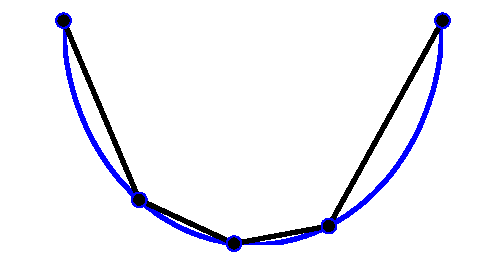
\includegraphics[width=0.3\textwidth]{figs/outer_approximation.pdf}
%\caption{With the 5 sample points $(X_i, h(X_i))$, the
%  black and the blue convex function represent equivalent fits. SCAM
%  chooses the inner piece-wise linear convex functions.}
%\end{SCfigure}

The sparse convex additive model optimization in \eqref{np} is a quadratic program with
$O(np)$ variables and $O(np)$ constraints. 
Directly applying a QP solver for $f$ and $\beta$
is computationally expensive for relatively large
$n$ and $p$. However, notice that variables in different feature
dimensions are only coupled in the squared error term
$(y_{i}-\mu - \sum_{k=1}^{p}f_{ik})^{2}$. Hence, we can apply the block
coordinate descent method, where in each step we solve the following
QP subproblem for $\{f_k, \beta_k\}$ with the
other variables fixed. In matrix notation, the optimization is
\begin{align}
\begin{split}
\min_{ f_k, \beta_k, \gamma_k} \;\;& \frac{1}{2n} \| \uds{r}_k - \uds{f}_k \|_2^2 
     + \lambda \gamma_k \label{opt:1d_compact} \\
 \textrm{such that } & P_k \uds{f}_k = \diag(P_k \bds{x}_k)  \uds{\beta}_k \\
   & D_k \uds{\beta}_k \leq 0 \\
   & -\gamma_k \mathbf{1}_n \leq \uds{f}_k \leq \gamma_k \mathbf{1}_n   \\
   & \mathbf{1}_n^\tran \uds{f}_k = 0 
\end{split}
\end{align}
where $\uds{\beta}_k \in \R^{n-1}$ is the vector $\uds{\beta}_k =
(\beta_{1k}, \ldots, \beta_{(n-1)k})^T$, and
$\uds{r}_{k} \in \R^n$ is the residual vector $\uds{r}_{k} = (y_i -
\hat\mu - \sum_{k' \neq k} f_{ik'})^T$.
In addition, 
$P_k \in \R^{(n-1) \times n}$ is a permutation matrix where the $i$-th
row  is all zeros except for the value $-1$ in position $\perm{i}$ and
the value $1$ in
position $\perm{i+1}$, and $D_k \in \R^{(n-2) \times (n-1)}$ is another
permutation matrix  where the $i$-th row is all zeros except for a
value $1$  in position $\perm{i}$ and a value $-1$ in position $\perm{i+1}$.  We denote by
$\diag( v )$ the diagonal matrix with diagonal entries $v$.
The extra variable $\gamma_{k}$ is introduced to impose the
regularization penalty involving the $\ell_{\infty}$ norm.  

% \begin{equation}
% \label{eqn:opt_1d}
% \begin{split}
%        \min_{\bds{h}_{k\cdot},\bds{\beta}_{k\cdot},\gamma_{k}} &
%              \ \frac{1}{2n}\sum_{i=1}^{n}\Bigl((Y_{i}-\bar{Y}
%                 -\sum_{r\neq{k}}f_{ri})-f_{ki}\Bigr)^{2} 
%                       + \lambda\gamma_{k} \\
%         \textrm{such that} & \ f_{k(i+1)} = f_{k(i)} + \beta_{k(i)}(x_{k(i+1)}-x_{k(i)}),\\
%         &\ \beta_{k(i+1)} \geq \beta_{k(i)}, \ -\gamma_{k}\leq f_{ki}\leq\gamma_{k}\\
%         &\  \sum_{i=1}^{n}f_{ki}=0, \ (\forall i).
% \end{split}
% \end{equation}

This QP
subproblem involves $O(n)$ variables, $O(n)$ constraints and a sparse
structure, which can be solved efficiently using optimization
packages. In our experiments we use {\sc mosek} (\href{http://www.mosek.com/}{www.mosek.com}).  We cycle through
all covariates $k$ from $1$ to $p$ multiple times until convergence.
Empirically, we observe that the algorithm converges in only a few
cycles. We also implemented an ADMM solver for \eqref{np}
\citep{Boyd:admm}, but found
that it is not as efficient as this blockwise QP solver.

After optimization, the function estimate for an input vector $\bds{x}$ is, according to \eqref{hyper},
\begin{equation}
\begin{split}
      \hat f(\bds{x}) & = \sum_{k=1}^{p} \hat f_k(x_{j})+ \hat \mu 
= \sum_{k=1}^{p}\max_{i} \Bigl\{\hat f_{ik}+ \hat \beta_{ik}(x_{k}-x_{ik})\Bigr\} +
      \hat \mu.
\end{split}
\end{equation} 

The univariate concave function estimation required in the DC stage is a straightforward
modification of optimization~\eqref{opt:1d_compact}. It is only
necessary to modify the linear inequality constraints so that the subgradients are
non-increasing: $\beta_{\perm{i+1}k} \leq \beta_{\perm{i}k}$.


\subsection{Alternative Formulation}
Optimization \eqref{np} can be reformulated in terms of the second
derivatives.  We exploit this form in our theoretical analysis. 

The alternative formulation replaces the order constraints
$\beta_{\perm{i+1}k} \geq \beta_{\perm{i}k}$ with positivity constraints, which
simplifies the analysis.  Define $d_{\perm{i}k}$ as the second
derivative: $d_{\perm{1}k} = \beta_{\perm{1}k}$, and $d_{\perm{i}k} = \beta_{\perm{i}k} -
\beta_{\perm{i-1}k}$ for $i > 1$. The convexity constraint is equivalent to the
constraint that $d_{\perm{i}k} \geq 0$ for all $i > 1$.

It is easy to verify that $\beta_{\perm{i}k} = \sum_{j \leq i} d_{\perm{j}k}$ and 
\begin{align*}
f_k(x_{\perm{i}k}) = & f_k(x_{\perm{i-1}k}) + \beta_{\perm{i-1}k}(x_{\perm{i}k} - x_{\perm{i-1}k}) \\
 =& f_k(x_{\perm{1}k}) + \sum_{j < i} \beta_{\perm{j}k} (x_{\perm{j}k} - x_{\perm{j-1}k}) \\
 =& f_k(x_{\perm{1}k}) + \sum_{j < i} \sum_{j' \leq j} d_{\perm{j'}k} (x_{\perm{j}k} - x_{\perm{j-1}k})\\
 =& f_k(x_{\perm{1}k}) + \sum_{j' < i} d_{\perm{j'}k} \sum_{i > j \geq j'} (x_{\perm{j}k} - x_{\perm{j-1}k}) \\
 =& f_k(x_{\perm{1}k}) + \sum_{j' < i} d_{\perm{j'}k} (x_{\perm{i}k} - x_{\perm{j'}k}).
\end{align*}
We can write this more compactly in matrix notation as
\begin{align}
\nonumber
\left[ \begin{array}{c}
f_k(x_{\perm{1}k}) \\
f_k(x_{\perm{2}k}) \\
\vdots \\
f_k(x_{\perm{n}k})
\end{array} \right] &=
\left[ \begin{array}{ccc}
    (x_{k1} - x_{\perm{1}k})_+ & \cdots & (x_{k1} - x_{\perm{n-1}k})_+ \\
    \cdots & & \\
    (x_{kn} - x_{\perm{1}k})_+ & \cdots & (x_{kn} - x_{\perm{n-1}k})_+ 
\end{array} \right]
\left[ \begin{array}{c}
    d_{\perm{1}k} \\
    \cdots \\
    d_{\perm{n-1}k}
\end{array} \right] + \mu_k \\[10pt]
& \equiv \Delta_k d_k + \mu_k
\end{align}
where $\Delta_k$ is a $n\times n-1$ matrix such that $\Delta_k(i,j) =
(x_{\perm{i}k} - x_{\perm{j}k})_+$, $d_k = (d_{\perm{1}k} ,\ldots,
d_{\perm{n-1}k})$, and $\mu_k = f_k(x_{\perm{1}k}) \mathbf{1}_n$.
Because $f_k$ has to be centered, $\mu_k = - \frac{1}{n}
\mathbf{1}_n^\tran \Delta_k d_k$, and therefore
\[
\Delta_k d_k + \mu_k \mathbf{1}_n = 
   \Delta_k d_k - \frac{1}{n} \mathbf{1}_n \mathbf{1}_n^\tran \Delta_k d_k = 
   \bar{\Delta}_k d_k 
\]
where $\bar{\Delta}_k \equiv \Delta_k - \frac{1}{n} \mathbf{1}_n \mathbf{1}_n^\tran \Delta_k$ is $\Delta_k$ with the mean of each column subtracted.

We can now reformulate \eqref{np} as an equivalent optimization program with only centering and positivity constraints:
\begin{align}
\min_{d_k}\;\; & \frac{1}{2n} 
       \Bigl\| Y - \sum_{k=1}^p 
              \bar{\Delta}_k d_k \Bigr\|_2^2 
               + \lambda_n \sum_{k=1}^p \|\bar{\Delta}_k d_k \|_\infty   
     \label{opt:alternate_opt} \\
\trm{such that}\;\;  & d_{\perm{2}k}, \ldots , d_{\perm{n-1}k} \geq 0  	
               \qquad \trm{(convexity).} \nonumber 
\end{align}

The decoupled concave postprocessing stage optimization is again
similar. Specifically, suppose $\hat{d}_k$ is the output of
optimization~\eqref{opt:alternate_opt}, and define the residual vector
\begin{equation}
\hat{r} = Y -
\sum_{k=1}^p \bar{\Delta}_k \hat{d}_k.
\label{eq:residual}
\end{equation}  
Then  for all $k$ such that $\hat{d}_k = 0$, the DC stage optimization is
formulated as
\begin{align}
  \min_{c_k}\;\; & 
      \frac{1}{2n} \Bigl \| \hat{r} - \Delta_k c_k \Bigr \|_2^2
      + \lambda_n \| \Delta_k c_k \|_\infty 
      \label{opt:alternate_opt_concave}\\
 \trm{such that }\;\; & c_{\perm{2}k}, \ldots, c_{\perm{n-1}k} \leq 0 \qquad \trm{(concavity).} \nonumber
\end{align}

We can use either the off-centered $\Delta_k$ matrix or the centered
$\bar{\Delta}_k$ matrix because the concave estimations are decoupled
and hence are not subject to non-identifiability under additive constants.

\begin{remark}
  In our analysis, we assume that an upper bound $B$ to
  $\| f^*_k \|_\infty$ is known, and that we constrain our estimate
  $\hat{f}$ to obey the same boundedness condition.  That is, for each
  $k$, we require that $\|\hat{f}_k\|_\infty \leq B$. This boundedness
  constraint can be easily added to our optimization program. In
  optimization~\eqref{opt:alternate_opt}, we can enforce the boundedness
  condition by adding $p$ constraints $\| \bar{\Delta}_k d_k
  \|_\infty \leq B$ for $k=1,\ldots,p$ (and similarly for
  optimization~\eqref{opt:alternate_opt_concave}). We emphasize that we
  use the boundedness constraint only in our theoretical analysis; 
  our experiments do not impose any such condition.
\end{remark}


% DO NOT CHANGE; RefTex variables -minx

%%% Local Variables: ***
%%% mode:latex ***
%%% TeX-master: "paper.tex" ***
%%% End: ***